\documentclass[twocolumn,jsaiac]{jarticle}
\bibliographystyle{jsai}
%!TEX encoding = UTF-8 Unicode

\usepackage{multirow}
\usepackage{jsaiac}
\usepackage{bm}
\usepackage[dvipdfmx]{graphicx}
\usepackage[hyphens]{url}
\usepackage{algorithm}
\usepackage{algorithmic}

\title{
    \jtitle{真のゴールデンクロスは存在するか?}
}

\author{
    \jname{37-147308 飯塚 修平}
}

\affiliate{
  \jname{東京大学大学院 工学系研究科 技術経営戦略学専攻}
}

\def\Style{``jsaiac.sty''}
\def\BibTeX{{\rm B\kern-.05em{\sc i\kern-.025em b}\kern-.08em%
 T\kern-.1667em\lower.7ex\hbox{E}\kern-.125emX}}
\def\JBibTeX{\leavevmode\lower .6ex\hbox{J}\kern-0.15em\BibTeX}
\def\LaTeXe{\LaTeX\kern.15em2$_{\textstyle\varepsilon}$}

\newcommand{\argmax}{\mathop{\rm arg~max}\limits}
\begin{document}
\maketitle
\section{はじめに}
近年、インターネット証券の普及によって個人投資家が容易に株取引に参加できるようになった。
国内では NISA と呼ばれる少額投資非課税制度が導入され、中長期投資促進への期待が寄せられている\cite{nisa}。
また、2007 年より東京証券取引所は株式の売買単位を 100 株に統一するよう指導しており、
単位が引き下げられたことによって少額で株を購入できる環境が整ってきた\footnote{
  売買単位の集約に向けた行動計画 - 日本取引所グループ \url{http://www.jpx.co.jp/equities/improvements/unit/tvdivq00000050ft-att/keikaku.pdf}}。

投資家は運用成績を向上させるために株価の分析を行うことがあるが、その方法は大きく{\bf ファンダメンタル分析}と{\bf テクニカル分析}のふたつに分けることができる。
ファンダメンタル分析では、理論株価に基づいて株価を予測して投資判断を行う。
財務諸表から計算される財務指標に加えて、ニュースや IR 情報などの情報をもとに株価を予測する定性的分析手法である。
一方、テクニカル分析では、移動平均線に基づいて投資判断を行う。
過去の時系列データをもとに株価の値動きを予測する定量的分析手法である\cite{ga}。

今後、ますます個人投資家の株取引が容易になると、別のフルタイムの仕事を持つ個人投資家の数も増えてくるものと考えられる。
しかし彼らは専業トレーダーとは異なり、時間的な制約によって様々な銘柄の株価を常時チェックすることは難しいため、ある程度自動化された売買システムが必要になる。
そこで近年注目を浴びているのが、一定の売買ルールにしたがって取引を行う{\bf システムトレード}と呼ばれる手法である\cite{short}。
システムトレードはアルゴリズムに基づいた取引を行うため、定性的なファンダメンタル分析を取引に組み込むことは難しい。
一方、テクニカル分析は定量的な株価データに基づいて行われるため、アルゴリズムとして記述さえできればシステムトレードに組み込むことができる。
したがって、今後ますますテクニカル分析の重要性が増してくるものと考えられる。

そこで本稿では、テクニカル分析手法の中でもシンプルで広く用いられている{\bf グランビルの法則}にしたがって株式の取引を行うエージェントを作成してシミュレーションを行い、
テクニカル分析が運用成績向上にもたらす効果を検証する。
直近 1 年間に国内で取引された上場株の値動きデータを用いて評価実験を行った結果、
ランダムに取引を行う場合と比べてテクニカル分析に基づいて取引を行うエージェントは有意に良い運用成績を収めることができなかった。
しかし、テクニカル分析は売買する対象の銘柄を絞り込む効果がある。また、多面的に値動きを見る機能を加える事によって、運用成績を向上することができる可能性を示すことができた。
本稿で示した評価実験の結果および考察は、システムトレードを活用する個人投資家の運用成績向上に貢献するものと考えている。

\section{関連研究}
定量的な株価データを対象にしたテクニカル分析を用いて、高い運用成績を収めるアルゴリズムを開発する研究はいくつか行われている。
杉本らは株価の時系列データに決定木学習を用いて、未来状態予測を行うアルゴリズムを開発している\cite{decisiontree}。
他にも遺伝的アルゴリズムや遺伝的プログラミングなどのメタヒューリスティクスを用いた機械学習による手法もいくつか提案されており\cite{ga, gp}、
株価予測はデータマイニングの分野でよく取り上げられる研究テーマのひとつである。

一方、ファンダメンタル分析にもデータマイニングを適用して自動化しようとする試みは行われている。
和泉らは、国際金融情報センター\footnote{公益財団法人 国際金融情報センター\url{http://www.jcif.or.jp/}}が公開する市場解説記事にテキストマイニングを用いることで、
取引判断を行うエージェントを作成した\cite{multiagent}。
ファンダメンタル分析を行うエージェントとテクニカル分析を行うエージェントが混合した人工市場におけるシミュレーション実験も行われている\cite{short}。

このように、データマイニングによって得られた知識をもとに、自動で高い運用成績を目指したエージェントを開発する試みは行われている。
しかし、その多くは時系列データに機械学習を適用したものであり、個人投資家が機械学習の手法に詳しくない場合は投資判断材料として活用しやすいものではない。

\section{グランビルの法則}
それに対して、株価データの目に見えるパターンに着目して取引タイミングを分析する手法としてグランビルの法則がある。
グランビルの法則は、過去の株価データの平均移動線を利用したものであり、日々の株価の推移と見比べることによって売買タイミングを決定するテクニカル分析のひとつである\cite{granville}。

グランビルの法則では、株を買うタイミングとして、{\bf ゴールデンクロス}を提案している。
ゴールデンクロスとは、短期の移動平均線が長期の移動平均線を下から上に突き抜けた点のことであり、
株価上昇の勢いが強いことを示唆するとされている。逆に、短期の移動平均線が長期の移動平均線を上から下に切った場合は、
株価の勢いが弱い{\bf デッドクロス}と言われ、売りのタイミングとされている\cite{goldencross}。

この定義はシンプルでわかりやすく、株価チャートを見るだけで当該の場所を発見しやすい。
そのため、データマイニングや時系列データ分析について詳しくない個人投資家にも使いやすいツールとして親しまれている。
こういった判断基準が明確な分析手法のほうが、投資の成否の原因がはっきりするため、投資というリスクがつきまとう活動に対する手法には向いていると考えられる。
そこで本稿では、このグランビルの法則、特にゴールデンクロスに着目して投資判断をした場合に、高い運用成績を収めることができることを検証する。

\section{評価実験}
評価実験では、戦略に基づいて売買を行うエージェントを作成してシミュレーションを行い、それらの平均利回りを比較してグランビルの法則の効果を検証する。
Algorithm \ref{simulation_algorithm}に、シミュレーション方法の概観を示す。
シミュレーションが$n$回繰り返される間、各エージェント$A$はランダムに選択された取引日$d$に対して、買い銘柄$b$を戦略に基づいて選択する。
そして、あらかじめ定めたられた売買スパン$s$後の株価の値上がり率$p_{d+s,b}/p_{d,b}$を計算する。
ただし、$p_{d,b}$は取引日$d$における銘柄$b$の株価を表すものとする。
その後、各エージェントが得られた平均値上がり率によって、パフォーマンスを評価する。
取引日$d$に対してランダムにひとつの買い銘柄を選択するベースラインエージェント$A_b$と、
取引日$d$にゴールデンクロスが発生している銘柄の中からひとつをランダムに選択する提案エージェント$A_p$を用意し、
そのパフォーマンスを比較する。
データは2014年9月18日から2015年7月6日の間に収集された国内で上場されている3616銘柄の日足株価データを用いた。
ゴールデンクロスの特定には 25 日移動平均線を用い、シミュレーション回数は$n=1000$、売買スパンは$n=25$日とした。
\begin{algorithm}
\caption{シミュレーションのアルゴリズム}
\label{simulation_algorithm}
\begin{algorithmic}
\REQUIRE シミュレーション回数 $n > 0$
\REQUIRE 売買スパン $s > 0$
\REQUIRE エージェント $A$
\FOR{$i=0$ to $n$}
\STATE 取引日$d$がランダムに選択される。
\STATE 各エージェント$A$は戦略に基づいて取引日$d$に買うべき銘柄$b$を選択する。
\STATE 取引日$d$における株価$p_{d,b}$を記録する。
\STATE 取引日$d+s$における値上がり率$p_{d+s,b}/p_{d,b}$を記録する。
\ENDFOR
\STATE 各エージェント$A$が生み出した平均値上がり率を比較する。
\end{algorithmic}
\end{algorithm}

実験結果を表\ref{tbl:result}に示す。提案エージェント$A_p$の平均利回りとベースラインエージェント$A_b$の平均利回りについてt検定による平均値の差の検定を行ったところ、
p値は0.76であり、有意な差が見られなかった。
提案エージェント$A_p$の選択銘柄数はベースラインエージェント$A_b$の選択銘柄数を下回っており、投資対象となる銘柄を絞り込む上ではゴールデンクロスに着目する戦略が有効に働いていることはわかる。
しかしその結果、ゴールデンクロスでの買い注文が利回りを改善する効果をもたらすことは確かめられなかった。
\begin{table}[htb]
\caption{各エージェントの平均利回り}
\label{tbl:result}
\begin{tabular}{c|c|c|c}
エージェント & 平均利回り & 分散 & 選択銘柄数 \\\hline\hline
ベースライン$A_b$ & 1.036 & 0.047 & 863 \\\hline
提案$A_p$ & 1.033 & 0.023 & 741\\\hline
\end{tabular}
\end{table}

\section{考察}
評価実験の結果を受けて、ゴールデンクロスに着目した取引きがランダムな取引に比べて利回りを向上させることができなかった原因を考察する。

\subsection{天井づかみ}
提案エージェントの投資判断の中で最も低い値上がり率を示したのは、(株)ブロッコリーを2014年12月22日に買い、2015年2月2日に売った取引きである
(図\ref{fig:broccoli}参照\footnote{株価チャートはすべてYahoo!ファイナンスから引用した。\url{http://stocks.finance.yahoo.co.jp/}})。
たしかにゴールデンクロスが発生しているものの、買い注文までの期間ずっと株価が上昇を続けている状態であり、一時急落して株価が反発した時に発生したゴールデンクロスであった。
株価が上昇した後に購入することは、それだけ割高な状態で株式を購入してしまう確率を大きくすることになる。
運用成績を向上させるためには、ゴールデンクロスの発生のみを見るのではなく、それまでの株価の推移のパターンも含めて考えることが必要になると考えられる。
\begin{figure}[htb]
\begin{center}
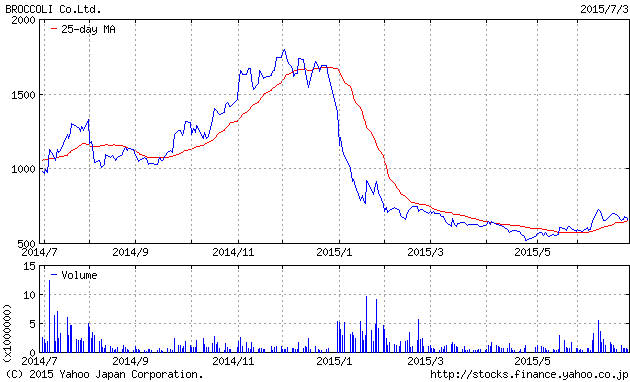
\includegraphics[width=8cm,clip]{broccoli.png}
\end{center}
\caption{(株)ブロッコリーの株価の遷移}
\label{fig:broccoli}
\end{figure}

一方、高い値上がり率を示したものに、(株)宮入バルブ製作所がある(図\ref{fig:miyairi}参照)。
2015年1月6日に発生したゴールデンクロスで購入することで、高いパフォーマンスを示すことができた。
ただし、こちらも(株)ブロッコリーと同様にゴールデンクロス以前はゆるやかの株価上昇のトレンドが進んでいた。
このことから、買いタイミングとして魅力的なゴールデンクロスとそうでないゴールデンクロスを判断するには、
それまでの株価の推移の傾きで示されるトレンドだけでなく、移動平均線との交差から見えるパターンやPER, PBRなどの財務指標も着目する必要があると考えられる。
\begin{figure}[htb]
\begin{center}
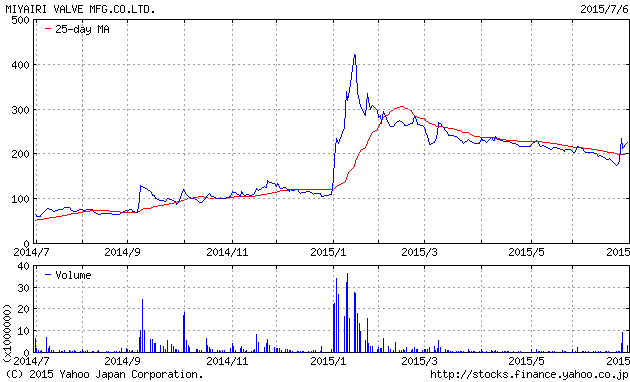
\includegraphics[width=8cm,clip]{miyairi.png}
\end{center}
\caption{(株)宮入バルブ製作所の株価の遷移}
\label{fig:miyairi}
\end{figure}

\subsection{売りのタイミング}
図\ref{fig:okinawa}に沖縄電力(株)の株価の推移を示す。2014年12月5日にゴールデンクロスが現れたが、2015年1月16日に売却した結果、損を出してしまった。
今回のシミュレーションでは売買のスパンを固定していたため、2015年1月以降の株価上昇のチャンスを逃してしまっている。
このことから、買いのタイミングと同様に売りのタイミングも重要であることがわかる。
デッドクロスが売りのタイミングとしてどの程度機能するのか、さらにゴールデンクロスとデッドクロスを組み合わせることでもたらされる運用成績への効果の検証は今後の課題としたい。
\begin{figure}[htb]
\begin{center}
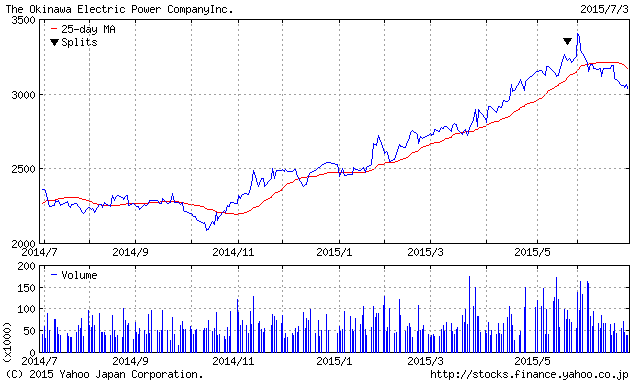
\includegraphics[width=8cm,clip]{okinawa.png}
\end{center}
\caption{沖縄電力(株)の株価の遷移}
\label{fig:okinawa}
\end{figure}

\section{まとめ}
本稿では、テクニカル分析手法のひとつであるグランビルの法則を取り上げ、
運用成績にもたらす効果を実際の株価データを用いたシミュレーションによって検証した。
買いタイミングを示すゴールデンクロスが現れた銘柄に対して取引きを行うエージェントと、
ランダムに取引きを行うエージェントの運用成績を比較した結果、その間には有意な差が見られなかった。
実験結果から、ゴールデンクロスだけではなく、その前に現れる推移のパターンや財務指標にも着目することが運用成績を向上する上で
重要な工夫になると考えられる。

\bibliography{references}
\bibliographystyle{jsai}

\end{document}
